\documentclass[12pt,a4paper]{article}

\usepackage[UTF8]{ctex}
\usepackage{amsmath,amscd,amsbsy,amssymb,latexsym,url,bm,amsthm}
\usepackage{amsfonts}
\usepackage{epsfig,graphicx,subfigure}
\usepackage{hyperref}
\usepackage{listings}
\usepackage[vlined,ruled,linesnumbered]{algorithm2e}
\usepackage{enumitem}
\usepackage{xcolor}
\usepackage{geometry}

%\uppercase\expandafter{\romannumeral1}:% 罗马数字。

\lstset{
language=Matlab,
keywordstyle= \color{blue!70},
commentstyle= \color{red!50!green!50!blue!50},
breaklines
}%设置listing插入语言

\setlength{\parindent}{0em}
\setlength{\parskip}{1em}

\geometry{bottom =3cm}
\newcommand{\textbi}[1]{%
\textbf{\textit{#1}}}

\newcommand{\ncolor}[1]{%
{\color[RGB]{139,117,0}{#1}}}
\newtheorem{theorem}{Theorem}[section]
\newenvironment{solution}{{\noindent \it \textbf{Solution:}}\\}

\title{MCM daily}
\author{Yunlong Cheng}

\begin{document}
\maketitle
\section{人工神经网络}
是由大量简单基本元件-神经元相互连接,模拟人脑神经处理信息的方式,进行信息并行处理和非线性转换的复杂网络系统。
\subsection{拓扑结构}
\begin{itemize}
  \item 网络层数。
  \item 各层神经元数量。
  \item 各神经元1之间相互连接的方式。
\end{itemize}
\subsection{激励函数}
三种形态:
\begin{enumerate}
  \item 阈值型:
  \begin{equation*}
    f(x) =
    \begin{cases}
      0 & x<0\\
      1 & x\ge 0 \\
    \end{cases}
  \end{equation*}
  \item 线性型(一般只用于输入神经元和输出神经元):$$f(x) = x$$
  \item S 型(常用于隐含层神经元):
    $$f(x) = \frac{1}{1+e^{-x}}$$ 或 $$f(x) = \frac{1-e^{-x}}{1+e^{-x}}$$
    其中 x 前可以带上参数。
\end{enumerate}
\subsection{常见神经网络理论}
\begin{enumerate}
  \item BP 网络基本数学原理:
  是多层前馈神经网络,源于网络训练中,调整网络权值的训练算法是反向传播算法(BP 学习算法)。
  \begin{center}
    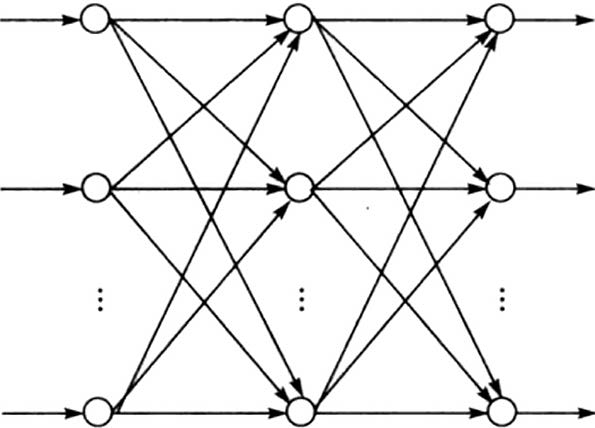
\includegraphics[width = 0.6\textwidth]{figures/3layer_illustrate.jpg}
  \end{center}
  BP 网络是一种具有三层或者三层以上的神经元的神经网络,包括输入层、中间层(隐含层)和输出层。其核心是数学中的\textbf{负梯度下降}理论,即 BP 网络的误差方向总是沿着误差下降最快的方向进行,常规三层 BP 网络权值和阈值调整公式如下:
  \begin{equation*}
    \begin{split}
      \omega_{ij}(t+1) = -\eta\frac{\partial E}{\partial \omega_{ij}} + \omega_{ij}(t) \quad& \omega_{jk}(t+1) = -\eta\frac{\partial E}{\partial\omega_{jk}} + \omega_{jk}(t)\\
      B_{ij}(t+1) = -\eta\frac{\partial E}{\partial B_{ij}} + B_{ij}(t) \quad& B_{jk}(t+1) = -\eta\frac{\partial E}{\partial B_{jk}} + B_{jk}(t)\\
    \end{split}
  \end{equation*}
\end{enumerate}
\end{document}
